\section{Introduction}

% What are agent based models? 
\par
Imagine you've just been given a massive raise and now earn significantly more than your neighbors. Is it be worth renovating your current property or should you move to a new place? How do expensive suburbs filled with people who earn more form?

\par
Below is an infographic of the median household income per county in the United States. You can see that the high income areas are clumped together in groups with the lower income areas surrounding them.

\par
There are many possible reasons for this clumping. A good way to look at a investigate these possible reasons is through the use of agent based models\cite{abm-wiki}. These models simulate simple behavior of agents in a simple environment to achieve a similar pattern to the real world.

% OR was it the very first
\par
Simulating population movements using agents is nothing new. Thomas C. Schelling's "Dynamic Models of Segregation", published in 1971, was among the first to do this. His model had two agents that both behaving the same way. They would move if they were "unhappy" because they were outnumbered by the other agent.

\par
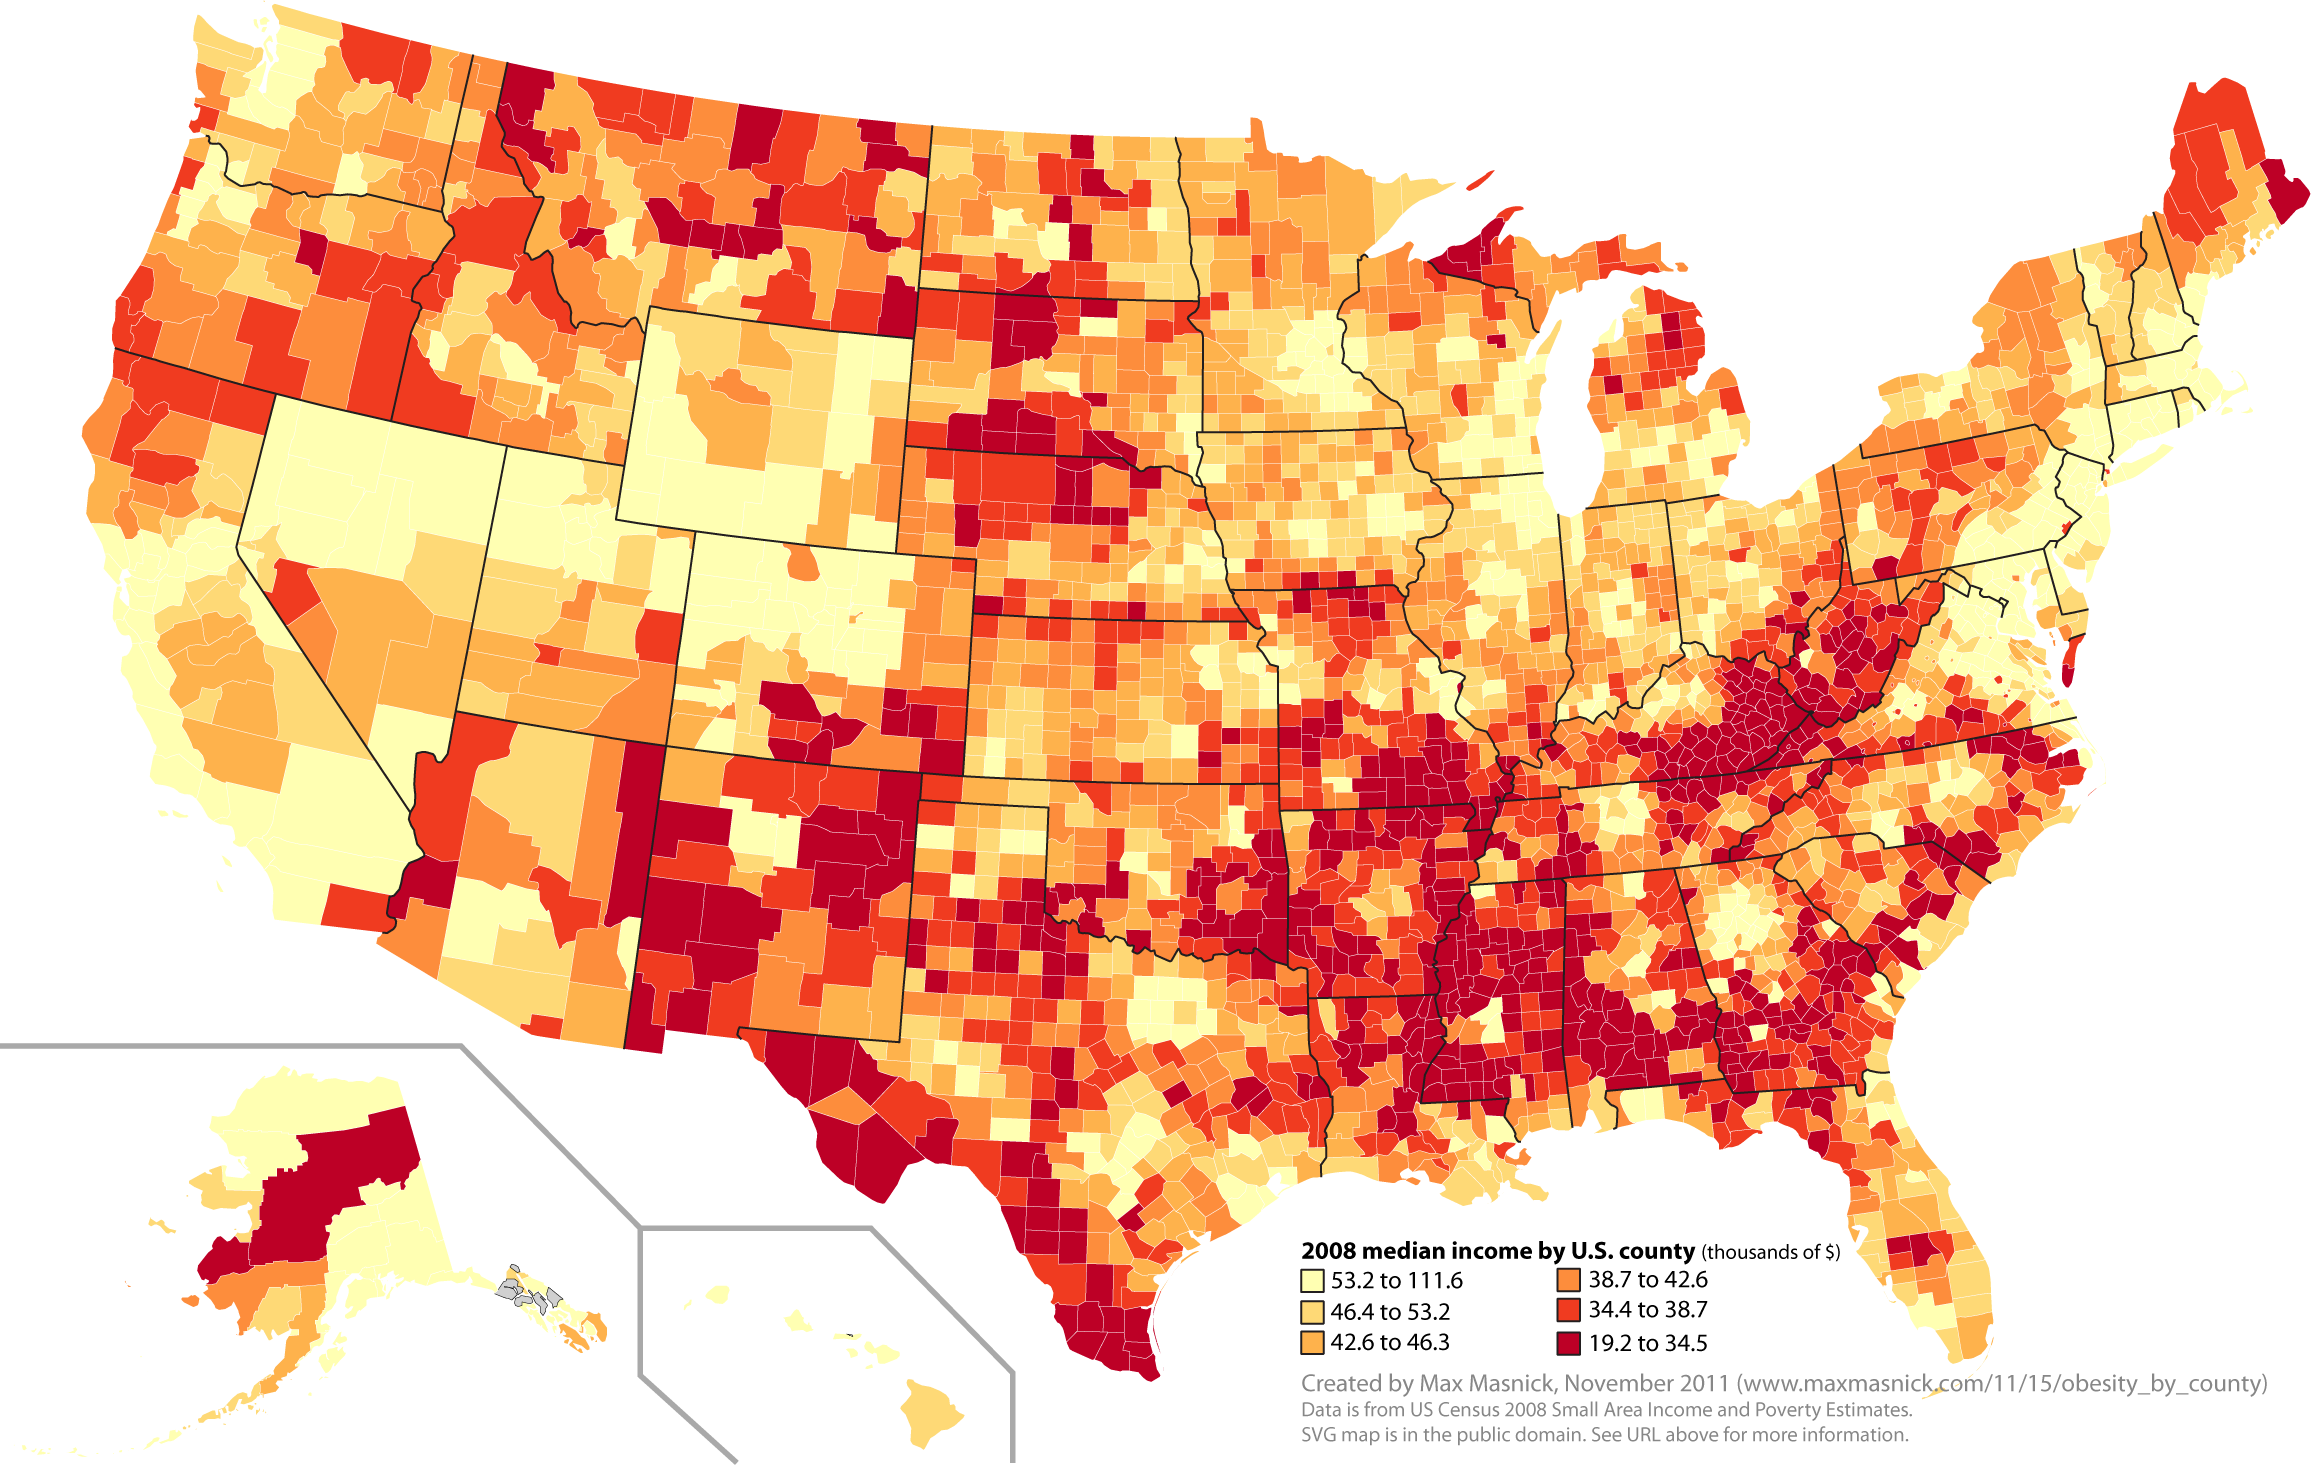
\includegraphics[width=15cm]{images/income_by_county_large_us}

%\par
%http://en.wikipedia.org/wiki/Agent-based\_model

